\chapter{Logo Retrieval System Evaluation}\label{c:evaluation}

This chapter evaluates the different solutions to detect and retrieve logos from images, detailed in chapter \ref{c:logoretrievalsystem}. Section \ref{s:explogodetection} compares the performance of different detectors and chooses the best performing for further usage. After that, the complete systems are evaluated in section \ref{s:logoretrieval}. Finally, the effect of training of the networks with classes, which are contained by the test set, will be examined.
\bigbreak
In order to get a holistic view on the performance of the complete retrieval system, the different solutions are evaluated by plotting the Detection and Identification Rate (DIR) as a function of average number of false positive classifications. DIR can also be considered as a multi-class recall, it involves not only the quality of the object detector, but also the classifier. In order to incorporate the probability scores of the detected logos, with the aim of reducing false positive recognitions, the final similarity scores between query and proposed regions are multiplied by that score.
\bigbreak
\section{Logo Detection}\label{s:explogodetection}

Although, there is not any known earlier work in the field of open-set logo detection and retrieval, it was still attempted to take a solution as baseline, which is already published. As chapter \ref{c:relatedwork} details, there exists a lot of research in improving the retrieval performance on the FlickrLogos-32 dataset using Faster R-CNN. Thereby, the region proposal network of a Faster R-CNN is chosen for logo detector baseline, which is trained only on the train and validation set of FlickrLogos-32. The network has almost state-of-the-art performance in closed-set logo retrieval, on the test set of this dataset. In particular with VGG-16 as base network, it yields 83.7 mAP, whereas the best already published result is 84.2 mAP proposed by \cite{Bao:2016:RCL:3007669.3007728}, using the multiscale Fast R-CNN approach and AlexNet, as base network.
\bigbreak
All the results of the following experiments are compared in figure \ref{f:detectioneval}. The data points are gathered by moving a threshold value on the region objectness probability emitted by the network.
Firstly, the RPN of the baseline network is evaluated on the Football-2 dataset, introduced in section \ref{ss:sportlogos}. Afterwards, the network is trained on all the publicly available logo datasets with bounding box annotations, introduced in section \ref{s:logodatasets}. Finally the improvement of the RPN network is tested. This network has already a better recall performance, but it retrieves much more false locations for lower threshold values.
Next, a class agnostic Faster R-CNN is trained again on all public datasets, but now only with "logo" class. Both the RPN and the classifier with regression layer at the end of the network are tested. The latter option is referred as "FC" on the figure \ref{f:detectioneval}, because of the fully connected layers accomplishing the classification and bounding box regression. A quite interesting result is here, that by training the same model on the same dataset but without specific brand labels, the detection performance of the region proposal network improves (see "Public Datasets RPN" versus "Public Datasets Class Agnostic RPN").

\begin{figure}
  \centering
  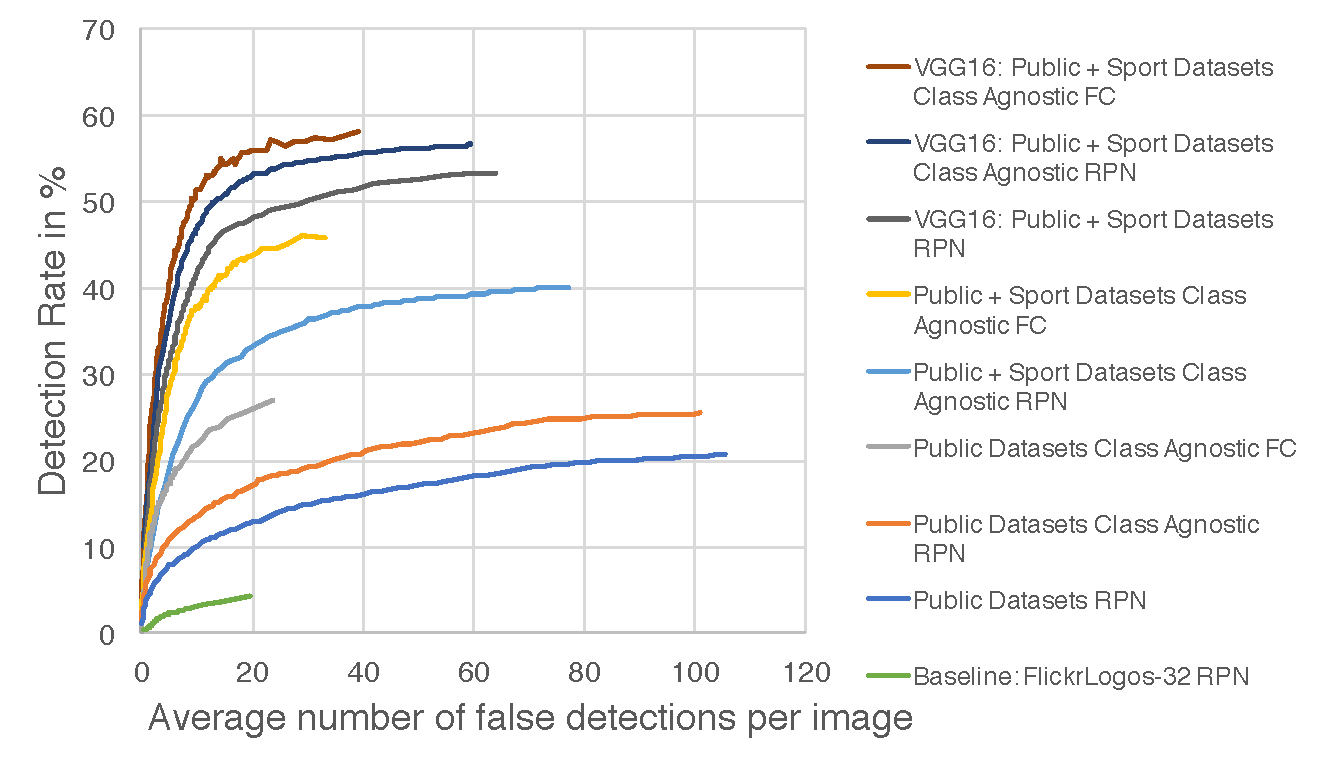
\includegraphics[width=120mm]{images/mt/logodetection.pdf}
  \caption{Logo detection evaluation}
  \label{f:detectioneval}
\end{figure}

In order to fine-tune the networks for the specific task, the datasets from similar domains were used, introduced in section \ref{ss:sportlogos}. The training is saturated after about one epoch of learning. This means, that the initial network is good pretrained for the task. This data has a large effect on the performance.
\bigbreak
Unfortunately, the test dataset contains a relatively small number of brands, which are already contained in the fused training dataset. Nevertheless, the effect of that is questionable. E.g. Adidas is one of the brands, which occurs both in the training set and with a large number on the video. On the other hand, Adidas logos are also included in the datasets FlickrLogos-32 and Logos32Plus and the networks, trained already on these datasets achieve much weaker results.
\bigbreak
Finally, a VGG-16 based Faster R-CNN was trained on all the training data, used earlier. Although, the gap between the RPN and the FC logo detector of this network became smaller, due to the much deeper base network before the RPN, the FC solution still yields superior performance both in recall and precision. One could argue, that the marginal improvement of FC to RPN does not worth the increased computational complexity. However, the RPN network has about double as much false positive on the same level of recall. This can cause much more additional computational burden for the classifier than what the FC layers do, especially if it needs large computational load.

The VGG-16 detector can generalize quite well, as figure \ref{f:extreme} shows, it is able to operate under extreme light conditions too.

\begin{figure}
  \centering
  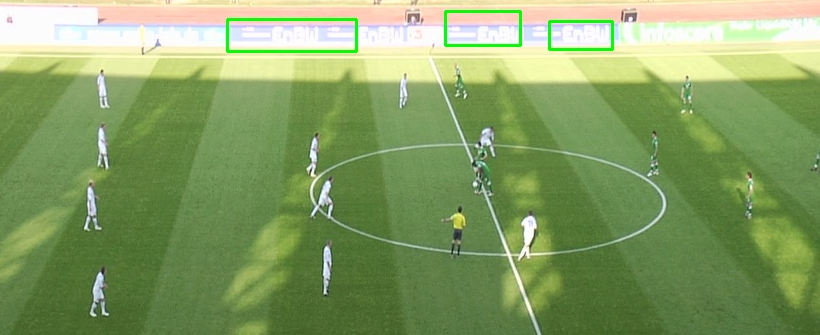
\includegraphics[width=120mm]{images/mt/extreme.png}
  \caption{Logo detection under extreme light conditions}
  \label{f:extreme}
\end{figure}

\section{Logo Retrieval}\label{s:logoretrieval}

After the best logo detector is found, the system should decide, which detections are relevant, and classify them, to the instances of the query set.

As a baseline system for logo retrieval, the same solution was chosen as for logo detection baseline - section \ref{s:explogodetection}, which is the Faster-Logos solution, detailed in section \ref{ss:solution1}. It consists of a Faster R-CNN, trained for logo detection on the train and validation set of FL-32.
\bigbreak
Nevertheless, this solution may be incapable of detecting the complete logo, especially if the logo has more distinct parts, as detailed in section \ref{ss:solution1}. The effect of mislocalization and the low size of output feature vector of the last layer is further investigated. To this end, the performance of the class probabilities was qualitatively tested. In particular, three logo images were tested from the same, unknown brand, having lesser or greater appearance variation:
\begin{itemize}
	\item a logo, cropped from a video,
	\item a logo with very similar background color, but in high resolution,
	\item a logo with a completely different color scheme also in high resolution.
\end{itemize}

The logos fill out the majority of the images, as figure \ref{f:confusion} shows. The assumption was, that despite of the unknownness of the brand, the descriptor features of the three logos will contain similar portion of probabilities of known brands, thus having low distance to each other. Unfortunately, the network was incapable to yield such feature vectors. The original logos and the most likely predicted logos from the known set can be seen in figure \ref{f:confusion}. The composition of the normalized features for the three query images is shown by figure \ref{f:fasterconfusion}.

\begin{figure}
  \centering
  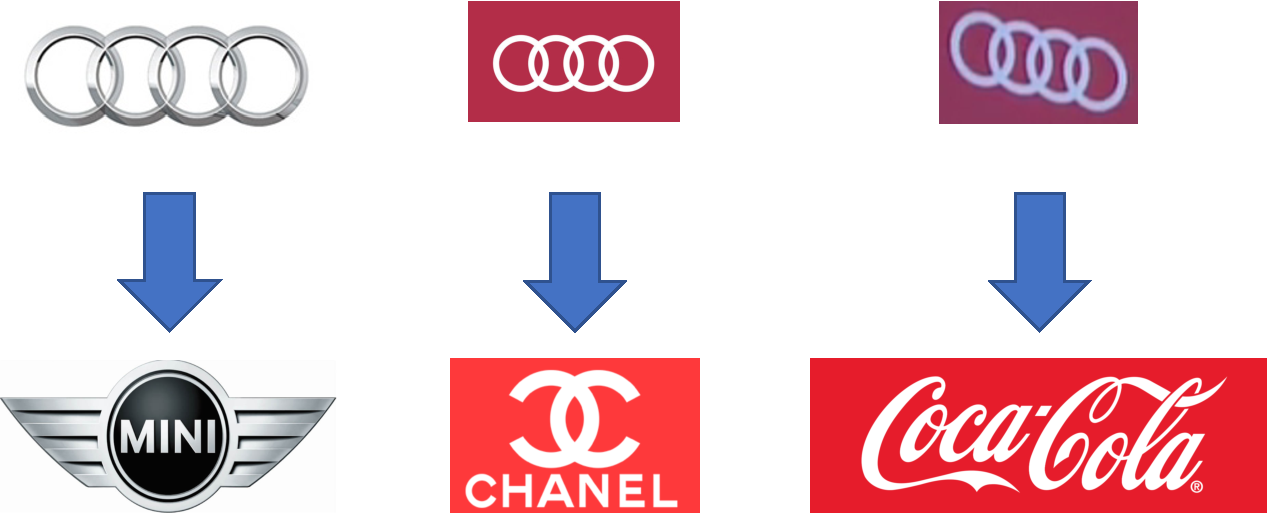
\includegraphics[height=40mm]{images/mt/confusion.pdf}
  \caption{Misclassification due to the small number of trained classes and data}
  \label{f:confusion}
\end{figure}

\begin{figure}
  \centering
  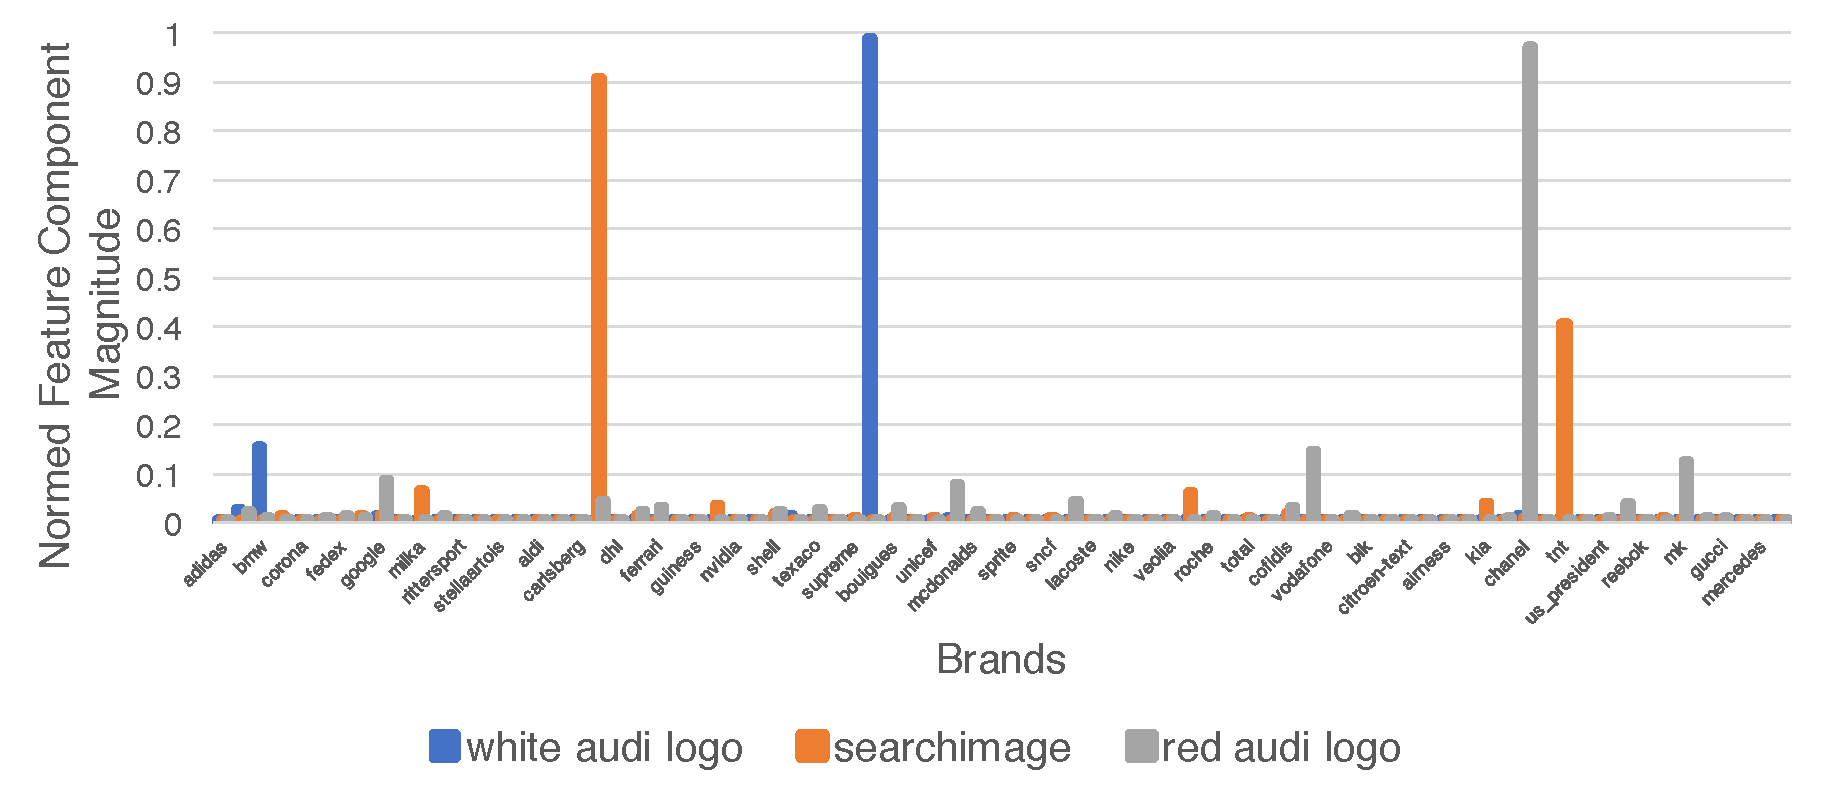
\includegraphics[height=60mm]{images/mt/faster_confusion.pdf}
  \caption{Feature vectors of the two query images and one cropped image from a video}
  \label{f:fasterconfusion}
\end{figure}

As section \ref{ss:solution2} details, the performance of this system may be improved by inferring the complete query image, instead of its most probable logo location. The system is evaluated on the Football-2 dataset, introduced in section \ref{ss:sportlogos}. For query set, logos from the videos were cropped. Because of the large intraclass variance shown in figure \ref{f:largevar}, multiple instances from some classes were chosen. But it is still a challenging task for the classifier, because of blur and different viewing angles of the logos in the search set.

\begin{figure}
  \centering
    \begin{tabular}{cccc}
      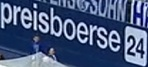
\includegraphics[width=25mm]{images/mt/largevar_1_b.jpg} &   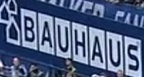
\includegraphics[width=25mm]{images/mt/largevar_2_a.jpg}  & 
\includegraphics[width=25mm]{images/mt/largevar_3_a.jpg} &   
\includegraphics[width=25mm]{images/mt/largevar_4_a.jpg} \\
      
\includegraphics[width=25mm]{images/mt/largevar_1_a.jpg} &   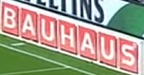
\includegraphics[width=25mm]{images/mt/largevar_2_b.jpg}  & 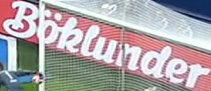
\includegraphics[width=25mm]{images/mt/largevar_3_b.jpg} &   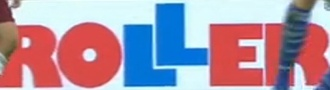
\includegraphics[width=25mm]{images/mt/largevar_4_b.jpg}
    \end{tabular}
  \caption{Samples for intraclass variation in sport videos. Images in the same columns have the same class.}
  \label{f:largevar}
\end{figure}
Occluded images are not included in the test set, because perhaps none of the TV-viewers would find the correspondence for unknown logos. Images, which have an edge size both in width and height smaller or equal than 25 pixel, are also omitted, because those very likely escape the viewer's attention. In addition, classes, having only one example, were removed, because in this case the query set would completely cover the ground truth set.

The similarities between the extracted feature vectors were calculated by cosine distance, and the output of the second last layer appeared to perform best as feature. The system is trained on all publicly available datasets. The low performance of the system is primarily induced by the classifier, which is weak in feature extraction from images with unknown classes. Thus, the network was additionally trained on the SportLogos dataset. This self annotated dataset induces a lot of new classes with very few ground truths, as shown in section \ref{ss:sportlogos}. Their instances may not be enough to completely train the classifier for those classes. Thus, it was questionable, whether the performance of the network enhances, if it is trained additionally also on the sport dataset. As figure \ref{f:sol2} shows, it yields better quality. It will be examined in the next paragraph, whether it is only due to the improvement of the RPN, or the classifier extracting better features. The performance of a random classifier is also indicated. This classifier assumed to work similarly as a real one, by outputting a class and a probability score for every region. Since it gets the ground truth regions as detections, it has a lower number of false positive classifications at the maximum of its recall, which is 2.5\% (there are 40 classes in the test set).
\begin{figure}
  \centering
  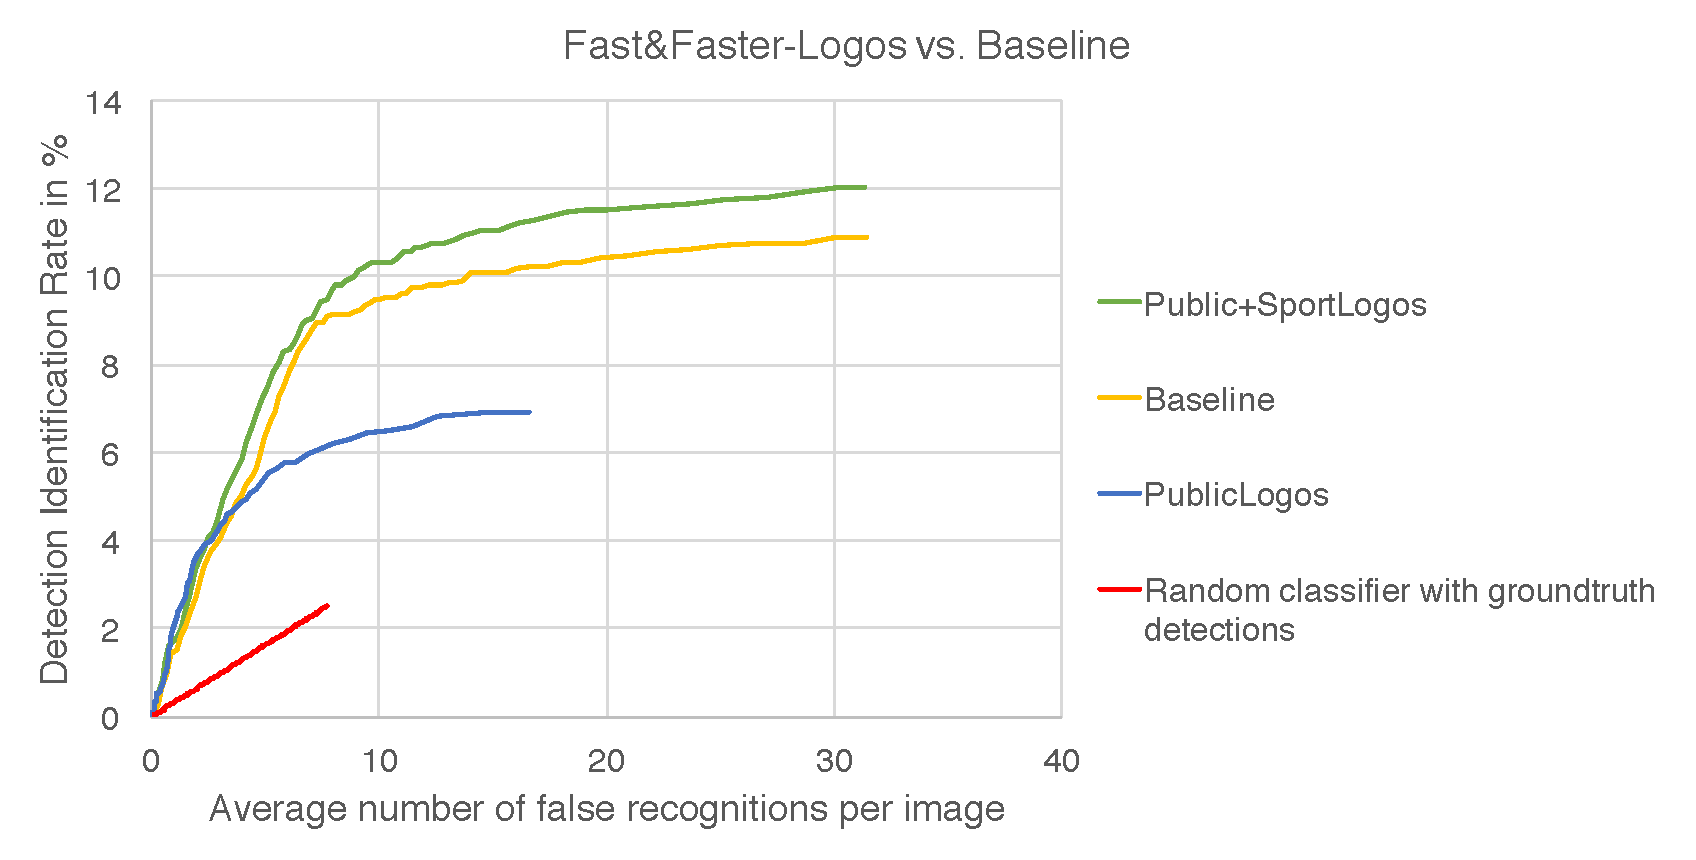
\includegraphics[height=60mm]{images/mt/sol2.pdf}
  \caption{Performance of Fast\&Faster-Logos compared with the Baseline and a Random Classifier}
  \label{f:sol2}
\end{figure}

The jointly trained classifier and detector, introduced in section \ref{ss:solution5}, did not seem to be useful for the case, if the ground truths are completely labeled with brand indication. Both branches were trained with the entire logo datasets, with and without brand label respectively. It achieved lower performance than the Baseline solution, which is trained on the same dataset. Figure \ref{f:sol5} shows the performance of this solution.
\begin{figure}
  \centering
  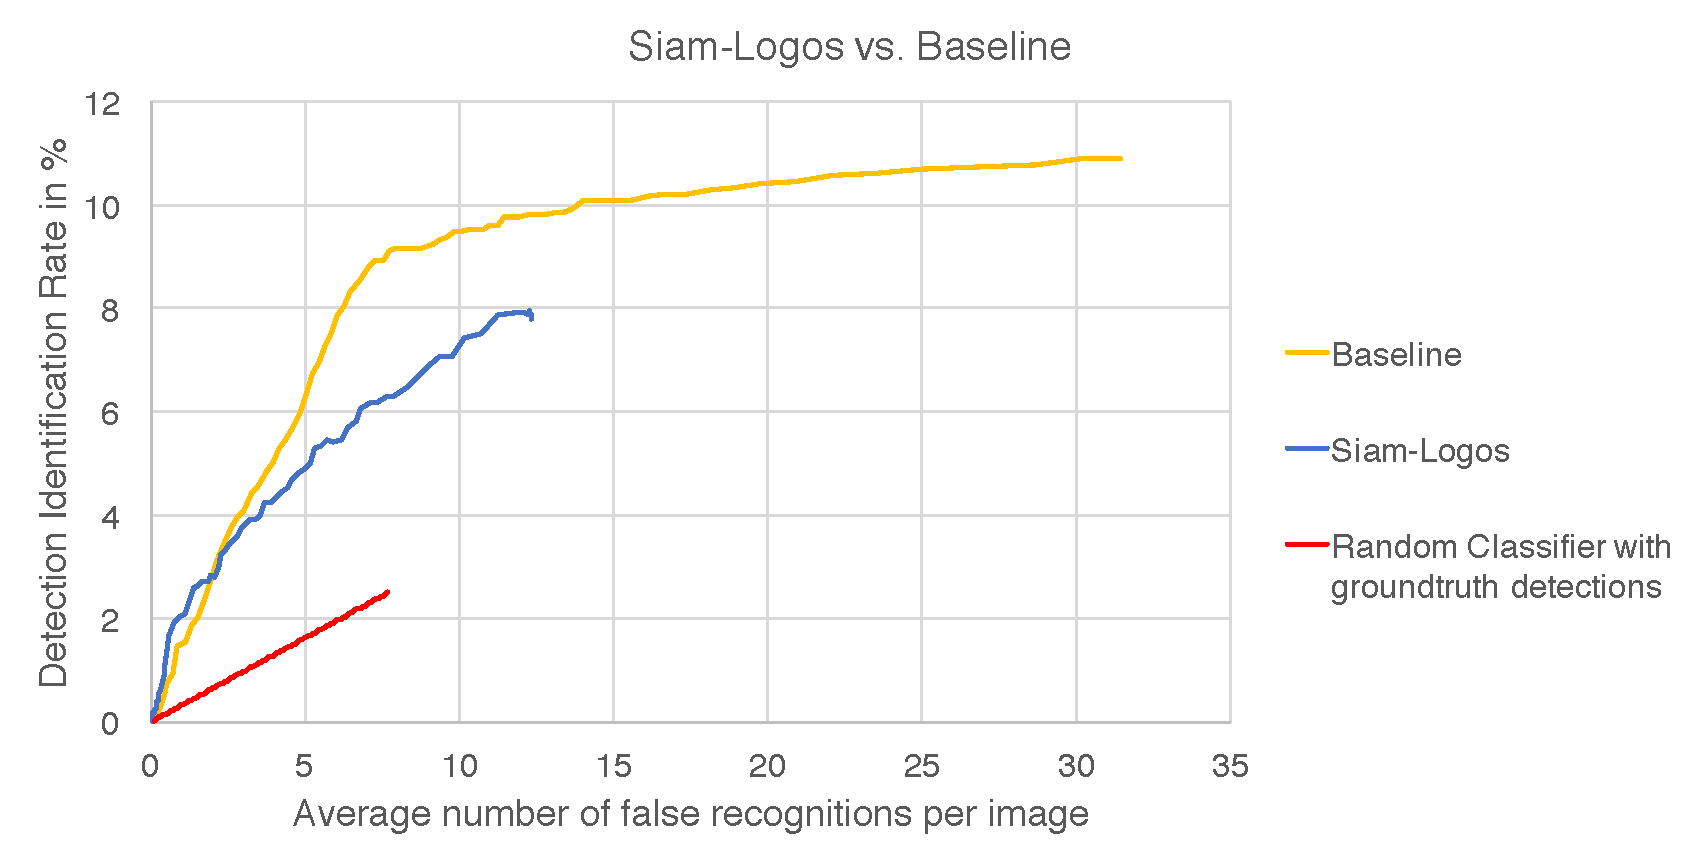
\includegraphics[height=60mm]{images/mt/sol5.pdf}
  \caption{Performance of Siam-Logos solution compared with the Baseline and a Random Classifier}
  \label{f:sol5}
\end{figure}
 As shown in section \ref{s:explogodetection}, a region proposal network may have inferior performance in logo detection compared to a class agnostic solution. Thus, the best performing FC logo detector can be applied, to ease the task of the classifier by yielding much fewer false positive detections. The features from the detections were then extracted with the same two networks as in the last paragraph, but now applied in fast R-CNN mode. Figure \ref{f:sol3} shows, that the system has a slightly better performance, but the classification power of the two networks is the same. This means, that the SportLogos dataset helped only in the detection task.
 \begin{figure}
  \centering
  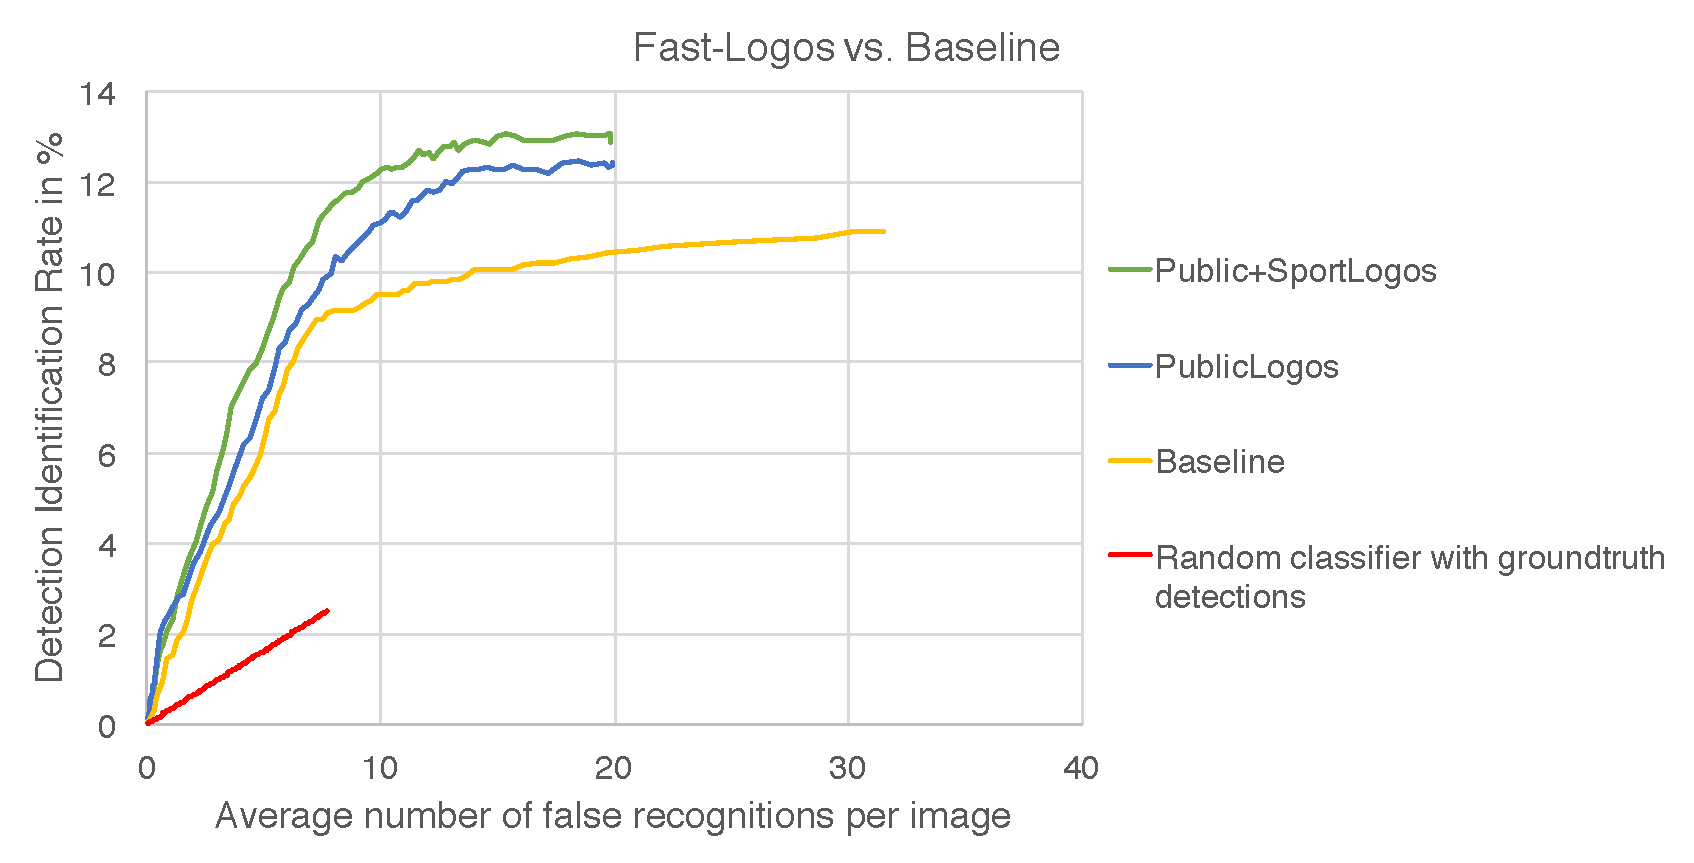
\includegraphics[height=60mm]{images/mt/sol3.pdf}
  \caption{Performance of Fast-Logos, i.e. replacing the RPN of a Faster R-CNN with a logo detector Faster R-CNN}
  \label{f:sol3}
\end{figure}

In order to achieve better classification performance, a feature extractor neural network can be placed after the logo detector, which is the idea of R-CNN, as shown in section \ref{ss:solution4}. The proposed bounding box regions are warped to 224x224 pixels, which is the conventional input size of these networks. No padding was used for the crops, so the aspect ratio was not preserved. However, this should not induce errors, because the query images undergo this aspect ratio change too. There were several feature extractor networks tested, and pretrained on ImageNet dataset by utilizing either the classification probabilities or the output of the second last layer. Figure \ref{f:sol4} summarizes their performance. Interestingly, the performance of the pretrained \texttt{VGG\_CNN\_M} network surpasses the pretrained ResNet. Additionally, there were two networks trained for classification on the data, cropped from all the logo datasets, preserving 10\% of it for validation:
\begin{itemize}
    \item A network \cite{ies_2016_herrmann_video_face_recognition} which is optimized for low resolution face recognition (32x32) thus, having the lowest inference time, among the evaluated feature extractor networks. This network could be utilized for logo recognition too, because of the logos, having low resolution on the videos. This network reached a classification accuracy of about 60\% on the validation data during training. The network was trained from scratch.
    \item A ResNet-50 network with reduced input size of 112x112. For this purpose, the last (5.) group of ResNet blocks was removed. This resolution is chosen because the network with input size of 224x224 was not able to converge. The reason for that could be the training data, having a much lower original average resolution of 137x102 (std.dev. 131x102). A network with this size is advantageous for the test dataset too, which has an average ground truth size of about 80x36 pixels (with std.dev of 47x20). Moreover, it is favourable also for the computation time. The weights of the network were initialized from the ImageNet pretrained ResNet-50 network. After training, it achieved 92\% accuracy on the validation set.
\end{itemize}
\begin{figure}
  \centering
  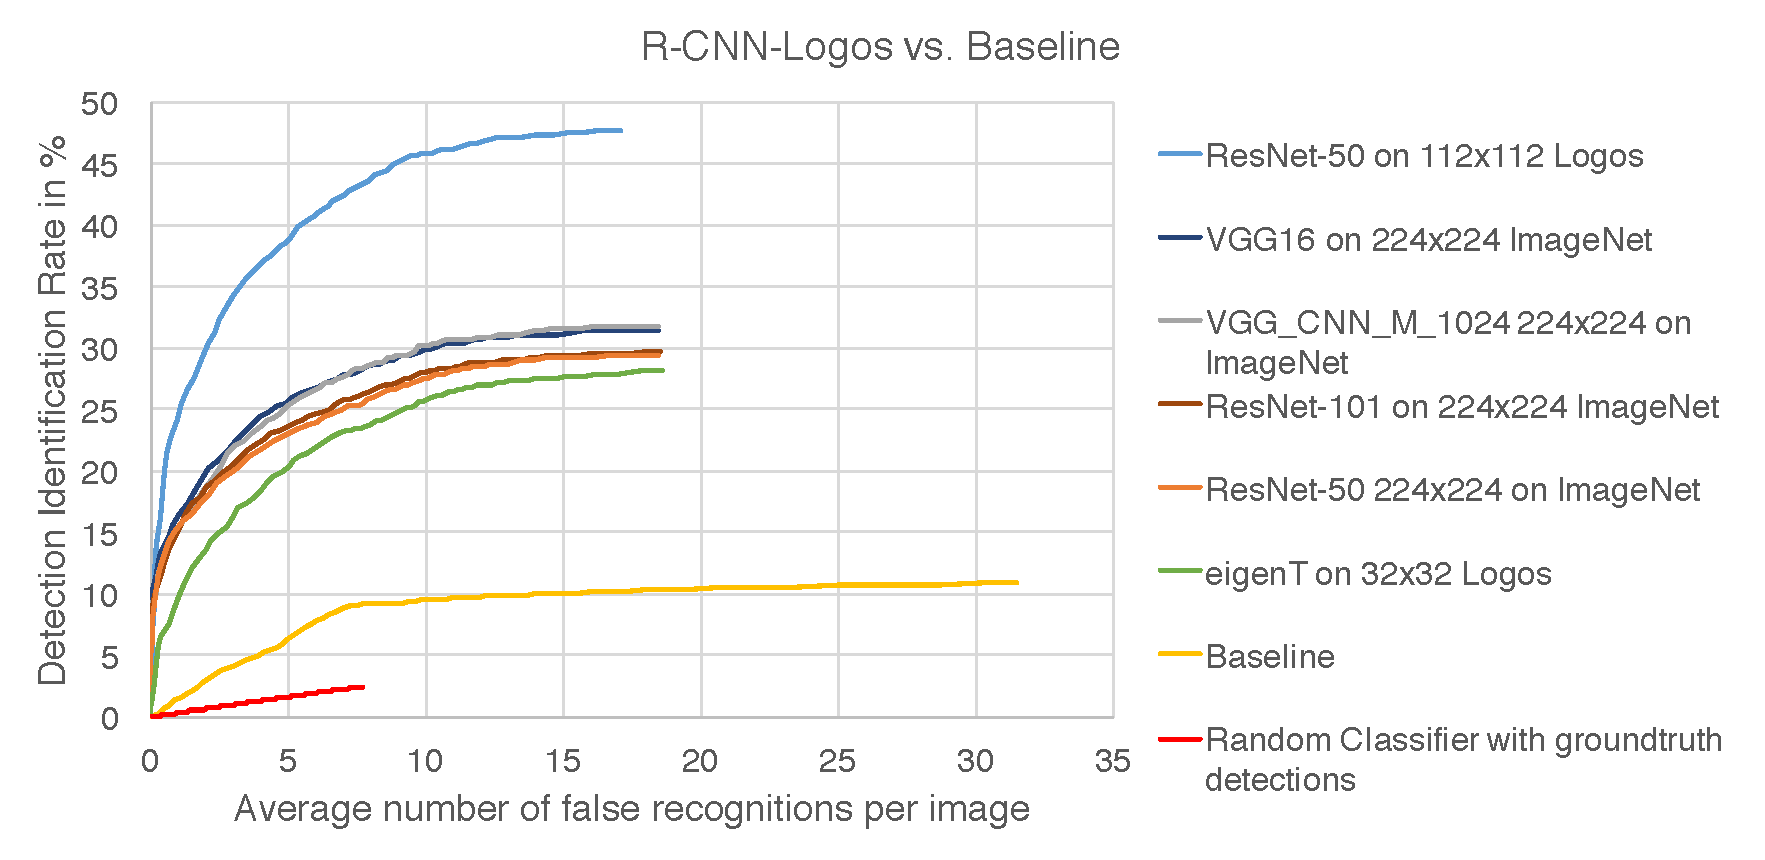
\includegraphics[height=60mm]{images/mt/sol4.pdf}
  \caption{Performance of the R-CNN-Logos solution by applying Faster R-CNN as region proposal system}
  \label{f:sol4}
\end{figure}


\section{Effect of Pretrained Classes}
Since the training dataset already contains some classes, which are part of the test dataset as shown in section \ref{ss:datasetfusion}, the effect of this data had to be examined. For that purpose, the best performing networks were taken into account, one pretrained on ImageNet, the other on all the logo datasets. Then, the DIR curves are plotted for the two intersecting classes, with significant examples in the training set. The curves are plotted this time with the number of false positive recognitions. The figure \ref{f:commonbrandseffect} shows the result of the experiment, whereas the performance on all the classes is plotted too, over the number of false positive recognition per brands for comparison reasons. The following conclusions can be drawn:
\begin{itemize}
    \item Pretraining with classes from the test set is less influential, as expected:
    \begin{itemize}
        \item Converging point of Adidas without pretraining (FP: 4)  DIR = 36. With pretraining DIR = 49.
        \item Converging point of VW without pretraining (FP: 27)  DIR = 55. With pretraining DIR = 60.
    \end{itemize}
    \item These two classes were much easier for the classifiers to retrieve, regardless the pretraining on the same classes.
    \item Although the false positive recognition with class pretraining is lower than the average, it is not significant.
    \item The number of false positive recognitions of the ImageNet network are much lower for low similarity thresholds. This could mean, that the network tends to choose pretrained classes for the detections, which could explain the additional misclassifications.
\end{itemize}
\begin{figure}
  \centering
  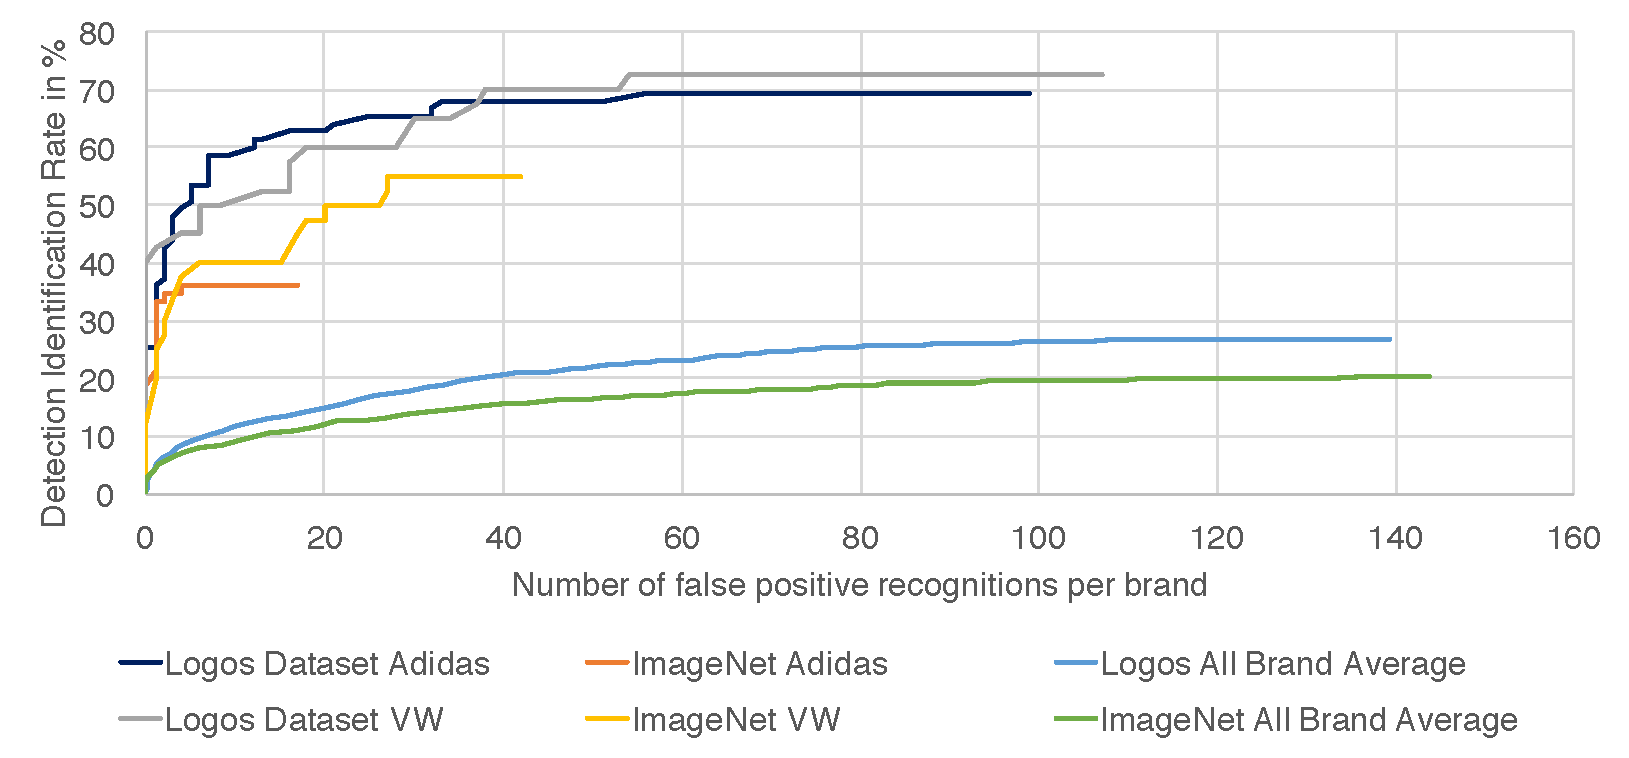
\includegraphics[height=60mm]{images/mt/commonbrandseffect.pdf}
  \caption{Effect of pretrained classes. The performance of a network, trained with and without the two classes, occurring in the test set, and the average performance of the networks.}
  \label{f:commonbrandseffect}
\end{figure}

\section{Perfomance evaluation}
To evaluate the feature extraction performance of the best system the output of the system is examined in detail. For this purpose, the output of the feature extractor network (the output of the last layer before softmax layer) is calculated for a crop image from the search set, which was misclassified, the query images of the real class, and the query image of the class, which was inferred incorrectly. The crop region was emitted by the detector network. The figure \ref{f:misclass} shows the crop from the query image in the middle, and the other query images around them. The similarity scores are indicated on the lines between the images, which was calculated with cosine distance. It can be seen, that the wrong query image has the greatest similarity score.
\begin{figure}
  \centering
  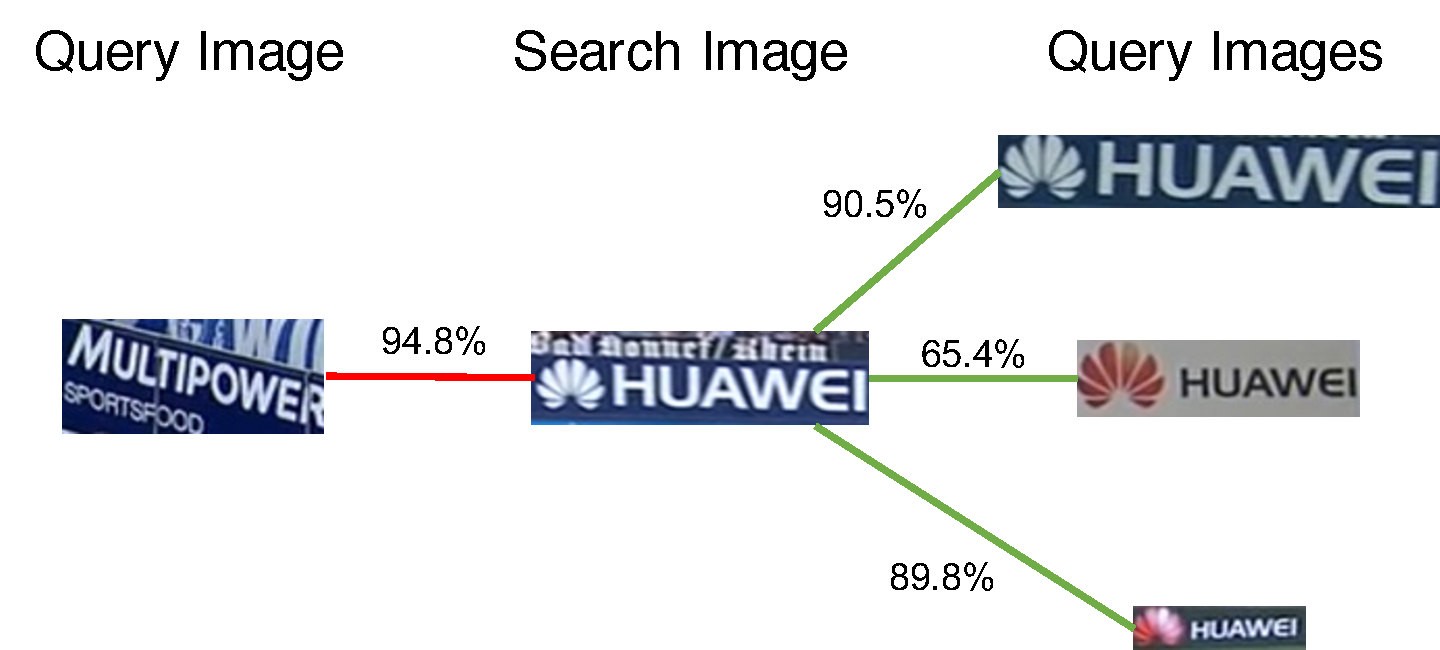
\includegraphics[height=60mm]{images/mt/misclass.pdf}
  \caption{Similarity scores between query images of two classes and a crop image from the search set (middle).}
  \label{f:misclass}
\end{figure}

\section{Retrieval times}
For the retrieval system not only the performance should be taken into account, but also the time needed to retrieve images. The average retrieval time per search image of every solution is measured and outlined in figure \ref{f:timebestdir} together with the achieved highest DIR value.
\begin{figure}
  \centering
  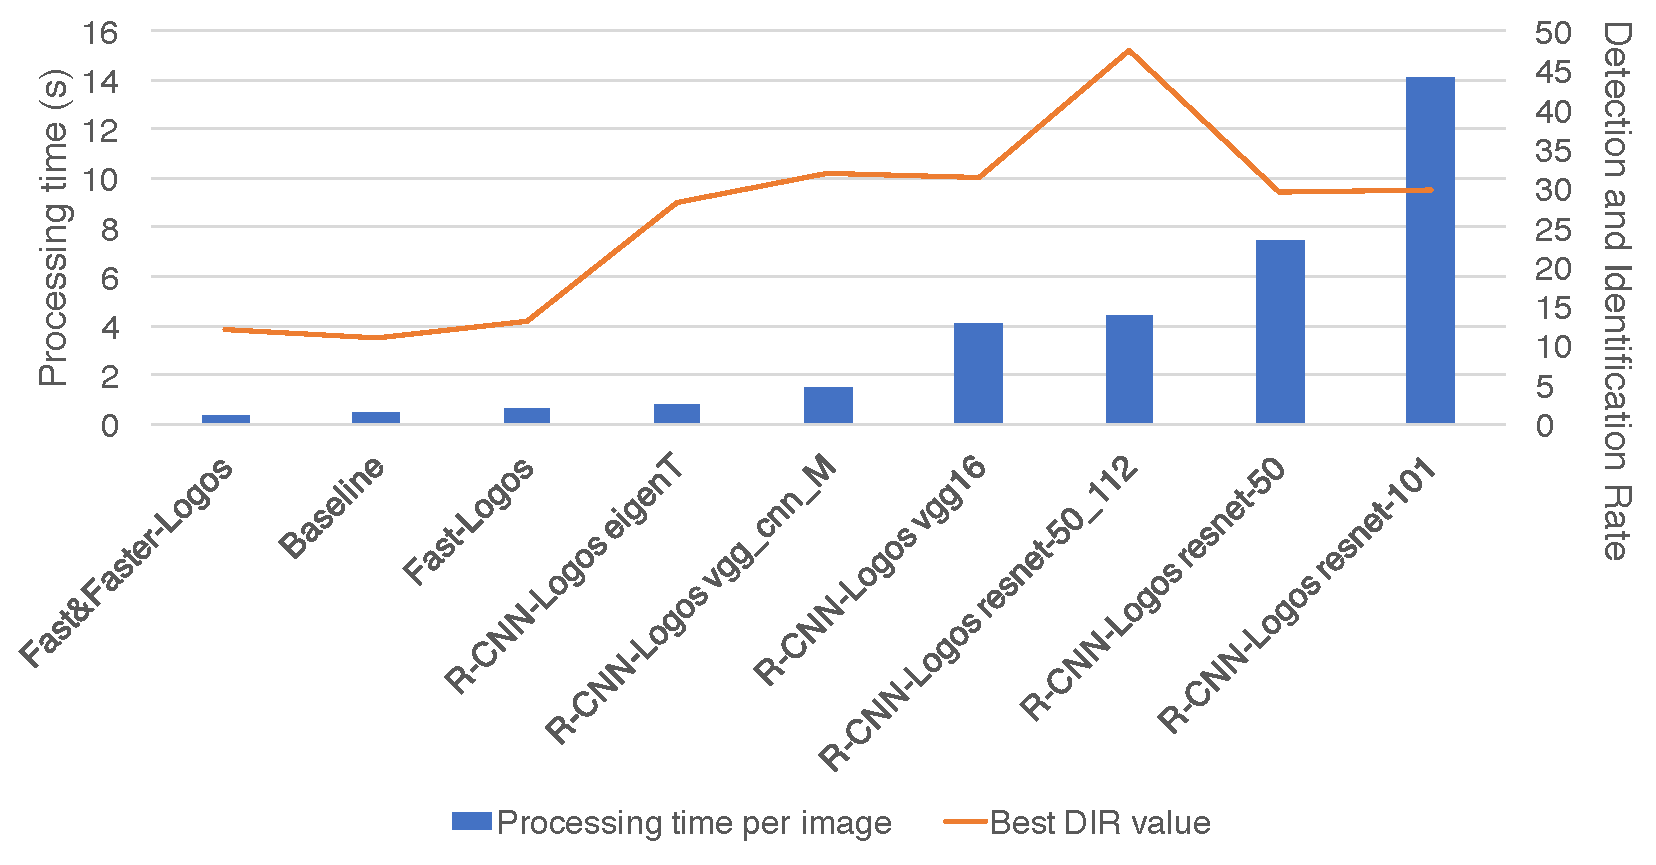
\includegraphics[height=60mm]{images/mt/timebestdir.pdf}
  \caption{Average processing time per image and the best achieved DIR value}
  \label{f:timebestdir}
\end{figure}
However, these data may not necessarily help to select the right system, according to the performance and time requirements. In order to combine the performance of the network and the average retrieval time, it was calculated, how much DIR value can be retrieved in one second with the different solutions. This evaluation was only accomplished for the R-CNN-Logos solutions, since these outperformed the other proposed systems with a large margin. The figure \ref{f:dirpertime} shows the result of this evaluation.
\begin{figure}
  \centering
  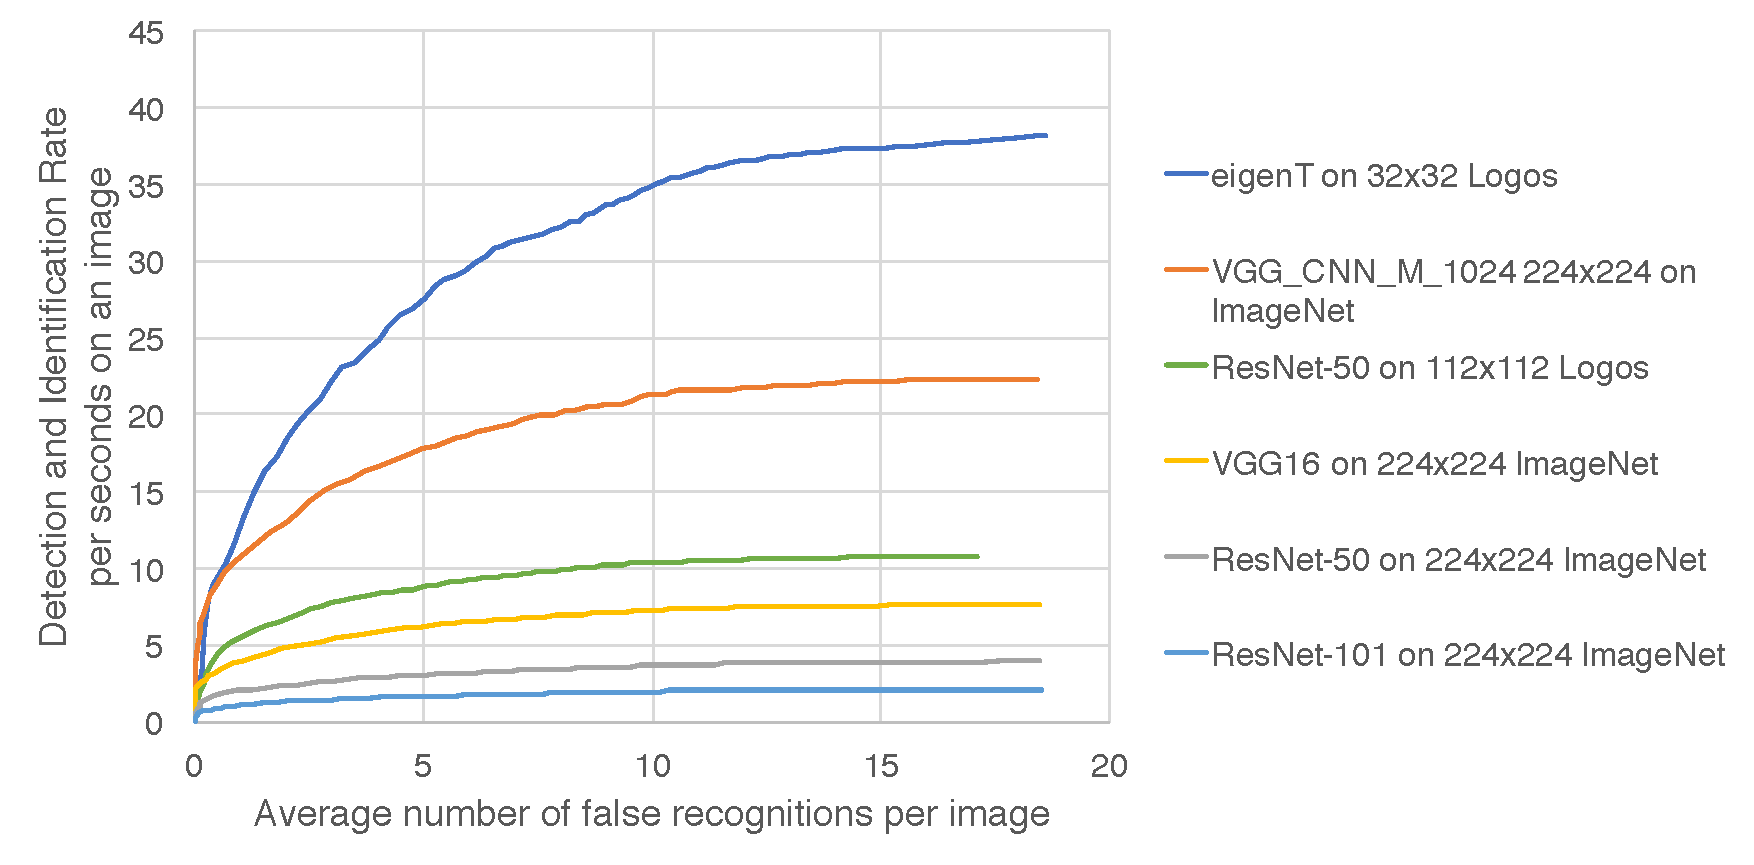
\includegraphics[height=60mm]{images/mt/dirpertime.pdf}
  \caption{Incorporating retrieval time and performance of the different networks of the solution R-CNN-Logos}
  \label{f:dirpertime}
\end{figure}